\section{Attention model details}
\label{sec:appendix_attention_model_details}

\begin{figure}[ht]
\vskip 0.2in
\begin{center}
\centerline{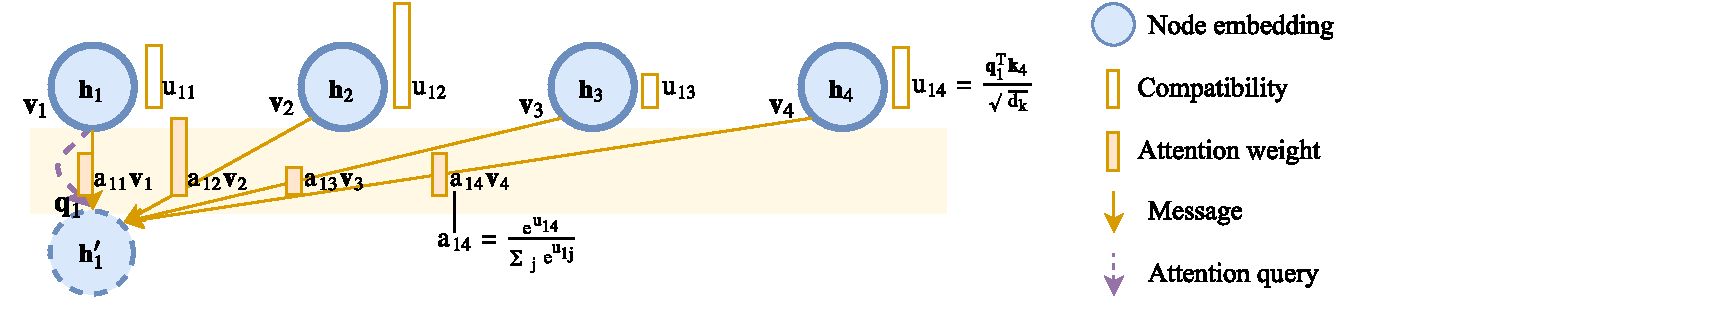
\includegraphics[trim={0 0 176 0},clip,width=\columnwidth]{./images/Attention}}
\caption{Illustration of weighted message passing using a dot-attention mechanism. Only computation of messages received by node $1$ are shown for clarity. Best viewed in color.}
\label{fig:attention_mechanism}
\end{center}
\vskip -0.2in
\end{figure}

\paragraph{Attention mechanism}
\label{sec:attention_mechanism}
We interpret the attention mechanism by \citet{vaswani2017attention} as a weighted message passing algorithm between nodes in a graph. The weight of the message \emph{value} that a node receives from a neighbor depends on the \emph{compatibility} of its \emph{query} with the \emph{key} of the neighbor, as illustrated in Figure \ref{fig:attention_mechanism}. Formally, we define dimensions $d_{\text{k}}$ and $d_{\text{v}}$ and compute the key $\mathbf{k}_i \in \mathbb{R}^{d_{\text{k}}}$, value $\mathbf{v}_i \in \mathbb{R}^{d_{\text{v}}}$ and query $\mathbf{q}_i \in \mathbb{R}^{d_{\text{k}}}$ for each node by projecting the embedding $\mathbf{h}_i$:
\begin{equation}
\label{eq:enc_qkv}
	\mathbf{q}_i = W^Q \mathbf{h}_i, \quad \mathbf{k}_i = W^K \mathbf{h}_i, \quad \mathbf{v}_i = W^V \mathbf{h}_i.
\end{equation}
Here parameters $W^Q$ and $W^K$ are $(d_{\text{k}} \times d_{\text{h}})$ matrices and $W^V$ has size $(d_{\text{v}} \times d_{\text{h}})$.
From the queries and keys, we compute the compatibility $u_{ij} \in \mathbb{R}$ of the query $\mathbf{q}_i$ of node $i$ with the key $\mathbf{k}_j$ of node $j$ as the (scaled, see \citet{vaswani2017attention}) dot-product:
\begin{equation}
\label{eq:compatibility}
	u_{ij} = \begin{cases}
		\frac{\mathbf{q}_i^T \mathbf{k}_j}{\sqrt{d_{\text{k}}}} & \text{if $i$ adjacent to $j$} \\
        -\infty & \text{otherwise.}
    \end{cases}
\end{equation}
In a general graph, defining the compatibility of non-adjacent nodes as $-\infty$ prevents message passing between these nodes. From the compatibilities $u_{ij}$, we compute the \emph{attention weights} $a_{ij} \in [0, 1]$ using a softmax:
\begin{equation}
	\label{eq:attention_weights}
    a_{ij} = \frac{e^{u_{ij}}}{\sum_{j'}{e^{u_{ij'}}}}.
\end{equation}
Finally, the vector $\mathbf{h}_i'$ that is received by node $i$ is the convex combination of messages $\mathbf{v}_j$:
\begin{equation}
	\label{eq:readout}
    \mathbf{h}_i' = \sum_{j} a_{ij} \mathbf{v}_j.
\end{equation}

\paragraph{Multi-head attention}
As was noted by \citet{vaswani2017attention} and \citet{velickovic2018graph}, it is beneficial to have multiple attention heads. This allows nodes to receive different types of messages from different neighbors. Especially, we compute the value in \eqref{eq:readout} $M = 8$ times with different parameters, using $d_{\text{k}} = d_{\text{v}} = \frac{d_{\text{h}}}{M} = 16$. We denote the result vectors by $\mathbf{h}_{im}'$ for $m \in {1, \ldots, M}$. These are projected back to a single $d_{\text{h}}$-dimensional vector using $(d_{\text{h}} \times d_{\text{v}})$ parameter matrices $W_m^O$. The final multi-head attention value for node $i$ is a function of $\mathbf{h}_1, \ldots, \mathbf{h}_n$ through $\mathbf{h}_{im}'$:
\begin{equation}
\label{eq:MHA}
	\text{MHA}_i(\mathbf{h}_1, \ldots, \mathbf{h}_n) = \sum\limits_{m=1}^{M} W_m^O \mathbf{h}_{im}'.
\end{equation}

\paragraph{Feed-forward sublayer}
The feed-forward sublayer computes node-wise projections using a hidden (sub)sublayer with dimension $d_{\text{ff}} = 512$ and a ReLu activation:
\begin{equation}
\label{eq:ff_layer}
	\text{FF}(\hat{\mathbf{h}}_i) = W^{\text{ff},1} \cdot \text{ReLu}(W^{\text{ff},0} \hat{\mathbf{h}}_i + \bm{b}^{\text{ff},0}) + \bm{b}^{\text{ff},1}.
\end{equation}

\paragraph{Batch normalization}
We use batch normalization with learnable $d_{\text{h}}$-dimensional affine parameters $\bm{w}^{\text{bn}}$ and $\bm{b}^{\text{bn}}$:
\begin{equation}
\label{eq:bn_layer}
	\text{BN}(\mathbf{h}_i) = \bm{w}^{\text{bn}} \odot \overline{\text{BN}}(\mathbf{h}_i) + \bm{b}^{\text{bn}}.
\end{equation}
Here $\odot$ denotes the element-wise product and $\overline{\text{BN}}$ refers to batch normalization without affine transformation.
